%% For double-blind review submission, w/o CCS and ACM Reference (max submission space)
\documentclass[10pt,conference]{ieeetran}%\settopmatter{printfolios=true,printccs=false,printacmref=false}

\usepackage{booktabs}   %% For formal tables:
                        %% http://ctan.org/pkg/booktabs
\usepackage{subcaption} %% For complex figures with subfigures/subcaptions
                        %% http://ctan.org/pkg/subcaption
\usepackage{amsmath,amsthm,amssymb}

\usepackage{xcolor,listings}

\usepackage{multirow}

\usepackage{stmaryrd}

\usepackage[noadjust]{cite}

\theoremstyle{definition}
\newtheorem{definition}{Definition}

\newif\ifdraft \drafttrue
\newif\iftext \textfalse
\newif\iflater \latertrue
\newif\ifaftersubmission \aftersubmissionfalse

% !!! PLEASE DON'T CHANGE THESE !!! INSTEAD DEFINE YOUR OWN texdirectives.tex !!!
\makeatletter \@input{texdirectives} \makeatother

%\IEEEoverridecommandlockouts
% The preceding line is only needed to identify funding in the first footnote. If that is unneeded, please comment it out.
\usepackage{cite}
\usepackage{amsmath,amssymb,amsfonts}
\usepackage{algorithmic}
\usepackage{hyperref}
\usepackage{graphicx}
\usepackage{textcomp}
\usepackage[capitalize]{cleveref}
\usepackage[inline]{enumitem}

\usepackage{xcolor}
\newcommand{\bcp}[1]{\ifdraft\textcolor{violet}{{[BCP:~#1]}}\fi}
\newcommand{\leo}[1]{\ifdraft\textcolor{teal}{{[LEO:~#1]}}\fi}
\newcommand{\apt}[1]{\ifdraft\textcolor{blue}{{[APT:~#1]}}\fi}
\newcommand{\rb}[1]{\ifdraft\textcolor{orange}{{[RB:~#1]}}\fi}
\newcommand{\sna}[1]{\ifdraft\textcolor{green}{{[SNA:~#1]}}\fi}
\newcommand{\COQ}[1]{\ifdraft\textcolor{red}{{[COQ DIFFERENCE:~#1]}}\fi}

\usepackage{listings}


\usepackage{xspace}
\newcommand{\cn}{\ifdraft\textsuperscript{\textcolor{blue}{[citation needed]}}\xspace\fi}

\makeatletter
\begingroup
\lccode`\A=`\-
\lccode`\N=`\N
\lccode`\V=`\V
\lowercase{\endgroup\def\memory@noval{ANoValue-}}
\long\def\memory@fiBgb\fi#1#2{\fi}
\long\def\memory@fiTBb\fi#1#2#3{\fi#2}
\newcommand\memory@ifnovalF[1]%>>=
  {%
    \ifx\memory@noval#1%
      \memory@fiBgb
    \fi
    \@firstofone
  }%=<<
\newcommand\memory@ifnovalTF[1]%>>=
  {%
    \ifx\memory@noval#1%
      \memory@fiTBb
    \fi
    \@secondoftwo
  }%=<<
\newcommand\memory@Oarg[2]%>>=
  {%
    \@ifnextchar[{\memory@Oarg@{#2}}{#2{#1}}%
  }%=<<
\long\def\memory@Oarg@#1[#2]%>>=
  {%
    #1{#2}%
  }%=<<
\newcommand*\memory@oarg%>>=
  {%
    \memory@Oarg\memory@noval
  }%=<<
\newcommand*\memory@ifcoloropt%>>=
  {%
    \@ifnextchar[\memory@ifcoloropt@true\memory@ifcoloropt@false
  }%=<<
\long\def\memory@ifcoloropt@true#1\memory@noval#2#3%>>=
  {%
    #2%
  }%=<<
\long\def\memory@ifcoloropt@false#1\memory@noval#2#3%>>=
  {%
    #3%
  }%=<<
\newlength\memory@width
\newlength\memory@height
\setlength\memory@width{23pt}
\setlength\memory@height{14pt}
\newcount\memory@num
\newcommand*\memory@blocks[2]%>>=
  {%
    \memory@num#1\relax
    \fboxsep-\fboxrule
    \memory@ifcoloropt#2\memory@noval
      {\def\memory@color{\textcolor#2}}
      {\def\memory@color{\textcolor{#2}}}%
    \loop
    \ifnum\memory@num>0
      \fbox{\memory@color{\rule{\memory@width}{\memory@height}}}%
      \kern-\fboxrule
      \advance\memory@num\m@ne
    \repeat
  }%=<<
% memory:
%  [#1]: width
%   #2 : count
%  [#3]: height
%   #4 : colour
%  [#5]: label
\newcommand*\memory%>>=
  {%
    \begingroup
    \memory@oarg\memory@a
  }%=<<
\newcommand*\memory@a[2]%>>=
  {%
    % #1 width
    % #2 count
    \memory@ifnovalF{#1}{\memory@width#1\relax}%
    \memory@Oarg\memory@height{\memory@b{#2}}%
  }%=<<
\newcommand*\memory@b[3]%>>=
  {%
    % #1 count
    % #2 height
    % #3 colour
    \memory@ifnovalF{#2}{\memory@height#2\relax}%
    \memory@oarg{\memory@c{#1}{#3}}%
  }%=<<
\newcommand*\memory@c[3]%>>=
  {%
    % #1 count
    % #2 colour
    % #3 label
    \memory@ifnovalTF{#3}
      {\ensuremath{\memory@blocks{#1}{#2}}}
      {\ensuremath{\underbrace{\memory@blocks{#1}{#2}}_{\text{#3}}}}%
    \endgroup
  }%=<<
\makeatother

\newcommand{\judgment}[2]{
  {\centering
  \vspace{\abovedisplayskip}
  \begin{tabular}{c}
    #1 \\
    \hline
    #2
  \end{tabular}
   \vspace{\abovedisplayskip}\par}}

\newcommand{\judgmentbr}[4]{
  {\centering
  \vspace{\abovedisplayskip}
  \begin{tabular}{c}
    #1 \\
    #2 \\
    #3 \\
    \hline
    #4
  \end{tabular}
   \vspace{\abovedisplayskip}\par}}


\newcommand{\judgmenttwo}[3]{
  {\centering
  \vspace{\abovedisplayskip}
  \begin{tabular}{c c}
    #1 & #2 \\
    \hline
    \multicolumn{2}{c}{#3}
  \end{tabular}
  \vspace{\abovedisplayskip}\par}}

\newcommand{\judgmentthree}[4]{
  {\centering
  \vspace{\abovedisplayskip}
  \begin{tabular}{c c c}
    #1 & #2 & #3 \\
    \hline
    \multicolumn{3}{c}{#4}
  \end{tabular}
  \vspace{\abovedisplayskip}\par}}

% Notational conventions
\newcommand{\HIGHSEC}{\textsc{HC}}
\newcommand{\LOWSEC}{\textsc{LC}}
\newcommand{\HIGHINT}{\textsc{HI}}
\newcommand{\LOWINT}{\textsc{LI}}
\newcommand{\IDS}{{\mathcal{I}}}
\newcommand{\ID}{I}
\newcommand{\ME}{\textsc{S}}
\newcommand{\NOTME}{\textsc{O}}
\newcommand{\TRANS}{\ensuremath{-}}
\newcommand{\JAL}{\ensuremath{\mathit{JAL}}}
\newcommand{\ACCYES}{\ensuremath{A}}
\newcommand{\ACCNO}{\ensuremath{I}}
\newcommand{\ACCCODE}{\ensuremath{K}}
\newcommand{\CRCALL}{\ensuremath{\mathit{CALL}}}
\newcommand{\CRRET}{\ensuremath{\mathit{RETURN}}}
\newcommand{\CRBOT}{\ensuremath{\bot}}
\newcommand{\VIS}{\textsc{vis}}
\newcommand{\HID}{\textsc{hid}}
\newcommand{\word}{w}
\newcommand{\addr}{a}
\newcommand{\WORDS}{{\mathcal W}}
\newcommand{\reg}{r}
\newcommand{\REGS}{{\mathcal R}}
\newcommand{\mach}{m}
\newcommand{\machT}{M}
\newcommand{\MACHS}{{\mathcal M}}
\newcommand{\MPT}{\mathit{MP}}
\newcommand{\obs}{o}
\newcommand{\obsT}{O}
\newcommand{\OBSS}{\mathit{Obs}}
\newcommand{\PC}[1]{\PCname(#1)}
\newcommand{\PCname}{\textsc{pc}}
\newcommand{\SP}{\textsc{sp}}
\newcommand{\pol}{p}
\newcommand{\POLS}{\mathcal{P}}
\newcommand{\pinit}{pinit}
\newcommand{\prop}{S}
\newcommand{\contour}{C}
\newcommand{\CONTOURS}{{\mathcal C}}
\newcommand{\component}{k}
\newcommand{\COMPONENTS}{{\mathcal K}}
\newcommand{\trace}{T}
\newcommand{\observer}{O}
\newcommand{\stateobs}{\sigma}
\newcommand{\seq}[1]{\overline{#1}}
\newcommand{\SEQ}[1]{\overline{#1}}
\newcommand{\dstk}[1]{{#1}.\mbox{\it stack}}
\newcommand{\dpcd}[1]{{#1}.\mbox{\it PCdepth}}
\newcommand{\ddep}[2]{{#1}.\mbox{\it depth}({#2})}
\newcommand{\dinit}{\mbox{\it Dinit}}
\newcommand{\empstack}{\mbox{\it empty}}
\newcommand{\access}[2]{\mbox{\it accessible}_{#1}({#2})}
\newcommand{\norm}[1]{\lvert{#1}\rvert}
\newcommand{\MPS}{\mathit{MPState}}
\newcommand{\mpstate}[2]{(#1,#2)}
\newcommand{\mpostate}[3]{(#1,#2,#3)}
\newcommand{\mpstatename}{mp}
\newcommand{\callmap}{cm}
\newcommand{\CALLMAPS}{\mathit{CallMap}}
\newcommand{\ret}[1]{\mathit{justret}\ #1}
\newcommand{\nextPC}{next}
\newcommand{\base}{b}
\newcommand{\stepsto}{\Longrightarrow}
\newcommand{\stepstounder}[1]{\stackrel{\mbox{\tiny{$#1$}}}{\Longrightarrow}}
\newcommand{\stepstounderfull}{\stepstounder{\textsc{RISCV}}}
\newcommand{\manystepsto}{\stepsto^\star}
\newcommand{\obstrace}{\mathit{obstrace}}
\newcommand{\funid}{f}
\newcommand{\FUNIDS}{\mathcal{F}}
\newcommand{\retmap}{\mathit{rm}}
\newcommand{\RETMAPS}{\mathit{RetMap}}
\newcommand{\codemap}{\mathit{fm}}
\newcommand{\CODEMAPS}{\mathit{FuncMap}}
\newcommand{\entmap}{\mathit{em}}
\newcommand{\ENTMAPS}{\mathit{EntryMap}}
\newcommand{\PUT}{\mathit{Until}}
\newcommand{\Trace}{T}
\newcommand{\traceelem}{a}
\newcommand{\TRACEELEMS}{A}
\newcommand{\head}{\mathit{head}}
\newcommand{\last}{\mathit{last}}

\newcommand{\stepstoobs}[1]{\xrightarrow{#1}}
\newcommand{\polstep}{\rightharpoonup}
\newcommand{\stepstopol}[1]{\overset{#1}{\rightharpoonup}}
%\newcommand{\stepstopol}[1]{\overset{#1}{\rightharpoonup}_P}

\newcommand{\stepplus}{\Rightarrow}
\newcommand{\stepkappa}{\Rightarrow_\kappa}
\newcommand{\induced}[2]{(#1, #2)^*}
\newcommand{\flows}{\sqsubseteq}
\newcommand{\flowsstrict}{\sqsubset}
\newcommand{\initmach}{\MACHS_{\mathit{init}}}
\newcommand{\initcontour}{\CONTOURS_{\mathit{init}}}
\newcommand{\closure}[1]{\textit{Close}#1}
\newcommand{\variant}[2]{\textit{Vars}(#1, #2)}
\newcommand{\isinf}{\mathit{inf}}

\newcommand{\Last}[1]{\mathit{Last}(#1)}

\newcommand{\HALT}{\textsc{HALT}}

\newcommand{\underscore}{\mbox{\_}}

\newcommand{\propdef}[1]{\text{\sc #1}}

\newcommand{\TRACE}[1]{\mathit{Trace}~(#1)}
\newcommand{\MTRACE}{\TRACE{\MACHS}}
\newcommand{\MOTRACE}{\TRACE{\MACHS \times \OBSS}}
\newcommand{\MPOTRACE}{\TRACE{\MACHS \times \POLS \times \OBSS}}


\makeatletter
\newcommand{\linebreakand}{%
  \end{@IEEEauthorhalign}
  \hfill\mbox{}\par
  \mbox{}\hfill\begin{@IEEEauthorhalign}
}
\makeatother

\begin{document}

%% Title information
\title{Formalizing Stack Safety as a Security Property}

\author{
  \IEEEauthorblockN{
    Sean Noble Anderson
  }
  \IEEEauthorblockA{
    Portland State University\\
    ander28@pdx.edu\\
  }
  \and
  \IEEEauthorblockN{
    Leonidas Lampropoulos
  }
  \IEEEauthorblockA{
    University of Maryland, College Park\\
    leonidas@umd.edu\\
  }
  \and
  \IEEEauthorblockN{
    Roberto Blanco
  }
  \IEEEauthorblockA{
    Max Planck Institute for Security and Privacy\\
    roberto.blanco@mpi-sp.org\\
  }
  \linebreakand
  \IEEEauthorblockN{
    Benjamin C. Pierce,
  }
  \IEEEauthorblockA{
    University of Pennsylvania\\
    bcpierce@cis.upenn.edu\\
  }
  \and
  \IEEEauthorblockN{
    Andrew Tolmach
  }
  \IEEEauthorblockA{
    Portland State University\\
    tolmach@pdx.edu\\
  }
}



%% Keywords
%% comma separated list
\ifcameraready
\keywords{Stack Safety, Micro-Policies}  %% \keywords are mandatory in final camera-ready submission
\fi

\maketitle

\section{The Setting}

We state our properties in terms of a generic machine subject to a few constraints,
but our examples and tests are focused on a RISC-V-like machine enhanced with PIPE,
a tag-based reference monitor. Importantly, such a machine has no explicit ``call''
instruction, only {\tt jal} instructions which may be used for that purpose or potentially
other purposes. Similarly, there is no ``return'', only {\tt jalr}, and so on.
We therefore define our properties under the assumption that we can distinguish the
steps that represent these abstract operations from those that do not -- an assumption
that is valid in our testing environment (Section [TBD]) and that is already necessary
to correctly apply tag-based enforcement in practice (cite something about this.)
\apt{This is too vague about how the  ``distinguishing'' can be performed.
  Should be clear up front that this will require annotating the code (at least
  in most cases).} 

The set of special operations that are recognized in this way are termed
{\it security operations}. Our properties are phrased as a {\it security semantics},
which extends the underlying machine with additional information\apt{``context''?}  about its
security principals and which registers and memory they require to be secure. This information\apt{``context''?}  evolves
dynamically through the execution of security operations.
Specifications \apt{of what?} may be
predicates on future states, e.g. assertions of the form
``When control returns to me...'', or relations on traces of future execution
(hyper-properties).

Unlike approaches that give a safe-by-construction semantics
for various security operations and then prove secure compilation to the underlying
enforcement mechanism, our machine is explicitly not safe unless the enforcement
is correctly instantiated; the security semantics gives us the means to judge whether
an enforcement scheme implements stack safety or not. 

We will first give a detailed example of a security semantics for a simple setting
in which our security operations are restricted to making calls and returns, and allocating
private memory within the current function activation. We then extend this model
to the full system that we test, which features:
\begin{itemize}
\item Function calls and returns, with caller- and callee-saved registers
\item Allocation of strictly private and strictly public regions on the stack
\item Arguments spilled onto the stack and/or passed by reference
\item Exceptions
\item Tail-call Elimination
\end{itemize}

Finally, we give a property definition for stack safety in which (some) stack-allocated
objects are governed by a provenance-based capability system, accessible only to those
functions which have recieved a valid pointer to them. \apt{ok for now, but may be more
  than can fit in the final paper}.

In section (TBD) we discuss the extension of this model into a simple concurrency setup.

\paragraph*{Threat Model}

We must trust that our method of distinguishing security operations is reasonable; if it
involves labels placed on code by a compiler, that means trusting that the compiler placed
those labels correctly. If it recognizes the operations based on the dynamic behavior of
the system, similarly, those definitions must be realistic.\apt{The substance of this paragraph
  is unclear. Isn't it implicit that any scheme must be ``reasonable'' to be useful?
  All the reader needs to know here is what assumptions we make; then they can decide whether they
  think these are reasonable or not.}

Otherwise, we do not assume that the code is reasonable or corresponds\apt{wrong word?} to any particular
calling convention or source construct. In particular, while we are agnostic as to the source
language, we certainly aim to support C, and so any source function might contain undefined
behavior resulting in its compilation to arbitrary machine code. A given enforcement
mechanism may place additional constraints, of course, particularly on the behavior of
call and return sequences.

In general, it is impossible to distinguish buggy source code from an attacker; in
our examples we will identify one function or another as an attacker, but we do not
require any static division between trusted and untrusted code, and aim to protect
even buggy code.

\apt{Need to discuss somewhere (maybe not here) what are the consequences of breaking our
  assumptions by mis-labeling code. Can we salvage anything? Do we care?}

This is a strong threat model, but hardware and timing attacks are out of scope,
and our properties are termination insensitive as a result of the enforcement mechanism
(below).

\paragraph*{Limitations}

Our concurrency model is fairly
simplistic, assuming a fixed number of threads each with its own dedicated processor.
We model memory safe stack objects, but not a heap. Regions outside of
stacks can be used however the compiler likes, including as a heap, but no protection is
built in and our properties assume that if a pointer to a stack object is stored there,
it is permanently compromised.

\subsection{The Basic Machine}

The building blocks of the machine are {\em words} and {\em registers}.
Words are ranged over by \(\word\) and, when used as addresses, \(\addr\),
and are drawn from the set \(\WORDS\) (by default\apt{??}, the set of 64-bit integers).
Registers are ranged over in general by \(\reg \in \REGS\), other than\apt{??} the
program counter \(\PCname\) and stack pointer \(\SP\).
They are divided into sets of caller-saved and callee-saved registers;
Figure \ref{fig:RISCVregs} gives an example division for a RISC-V machine as will
appear in our examples and testing, along with the register names that will appear in
example code, and their default security class (explained below).

\begin{figure}
  \begin{tabular}{| l | l | l |}
    \hline
    Set / & Names & Purpose \\
    Class & & \\
    \hline
    \(\mathit{CLR}\) / & {\tt t0} -- {\tt t6} & Caller-saved temps \\
    \(\unsealed\) & {\tt a0} -- {\tt a1} & Caller-saved args / return vals \\
    & {\tt a2} -- {\tt a7} & Caller-saved args \\
    \hline
    \(\mathit{CLE}\) / & {\tt s0} -- {\tt s7} & Callee-saved \\
    \(\sealed\) & {\tt ra} & Return Address \\
    & {\tt sp} & Stack Pointer \\  
    \hline
    \(\mathit{PUBLIC}\) / & {\tt pc} & Program Counter \\
    \(\public\) & & \\
    \hline
  \end{tabular}
  \caption{RISC-V register set}
  \label{fig:RISCVregs}
\end{figure}

Collectively addresses and registers are {\em state elements} \(\component\)
in the set \(\COMPONENTS ::= \WORDS + \REGS\).
%
{\em Machine states} are drawn from a set \(\MACHS\) ranged over by \(\mach\)
that defines a mapping \(\mach[\component]\) from state elements to values\apt{which are what? $\WORDS$, right?}.
{\em Events} are drawn from a set \(\OBSS\) and ranged over by \(\obs\).
\apt{Maybe want to mention $\tau$ now?}
The machine step function
\(\mach \xrightarrow{\overline{\psi}} \mach', \obs \in \MACHS \rightarrow
\MACHS \times \mathit{list} ~ \Psi \times \OBSS\)
is labeled by an ordered list of security operations, defined below,
and an event.\apt{Maybe put $\obs$ above the arrow too, as that is traditional.}
While the tag-based enforcement mechanism may cause the machine to
failstop, we model this as the machine silently diverging by remaining in the
same state. Since failstops are not distinguished from normal execution,
our properties will suffer the limitations typical of
{\it termination insensitive} systems \cite{}.\apt{better, but will need fuller
  explanation later}

For convenience, we will abbreviate multiple updates of a mapping
\(\mach[\component_0 \mapsto \word_0][\component_1 \mapsto \word_1]\dots\)
as \(\mach \llbracket A \mapsto B | C \rrbracket\), where \(A\) and \(B\)
are fomulae with free variables bound to sets in \(C\).

\subsection{Security Operations, Principals, and Security State}

Security operations consist of calls (including tailcalls), returns,
allocations and deallocations. Calls and tailcalls identify the address of the call's target,
and the argument registers. Allocations and deallocations are phrased in terms of a pair
of an offset \apt{from what?} and a size. Returns don't require any additional information.
%
\begin{align*}
  \psi \in \Psi ::= & \mathbf{call} ~ \addr_{target} ~ \overline{\reg_{args}} \\
  | & \mathbf{tailcall} ~ \addr_{target}  ~ \overline{\reg_{args}} \\
  | & \mathbf{return} & \\
  | & \mathbf{alloc} ~ \mathit{off ~ sz} & \mathit{off, sz} \in \mathbb{N} \\
  | & \mathbf{dealloc} ~ \mathit{off ~ sz} & \mathit{off, sz} \in \mathbb{N} \\
\end{align*}
%
Security principals are function activations: at any given time, the current
activation, and some number of pending ones.\apt{?? Is the principal an activation or
  a call stack (as defined below)?} Each activation has a {\it view}
of the system that maps each state element to a{\it security classe}:
\[sc \in SEC ::= \sealed | \unsealed | \object | \public\]
\[V \in \mathit{VIEW} ::= \COMPONENTS \rightarrow SEC\]

A view indicates, from the perspective of a given principal, whether an element is
private to an inactive principal (\(\sealed\)),
in an allocated object that is accessible to the current principal (\(\object\)),
available to be allocated (\(\unsealed\)), or
always accessible (\(\public\)).
The {\it initial view} \(V_0\) maps all stack locations to \(\unsealed\),
all other locations to \(\public\), and registers based on which set they
belong to (Figure \ref{fig:RISCVregs}): \(\sealed\) for callee-saved,
\(\unsealed\) for caller-saved, and \(\public\) otherwise.

A pending activation also carries the addresses to which the program counter
and stack pointer should point in the event of a return.
We represent a {\it call stack} \apt{``context'' ?} as a pair of the current activation's view
and a list of pending ones.
The initial call stack is \(\context_0 = (V_0, [ ~ ])\).
\[(V, \addr_{ret}, \addr_{sp}) \in \mathit{PEND} ::= \mathit{VIEW \times \WORDS \times \WORDS}\]
\[\context \in \CONTEXTS ::= \mathit{VIEW \times list ~ PEND}\]

Every security operation manipulates the call  stack via a function
\(Op : \Psi \rightarrow \MACHS \rightarrow \CONTEXTS \rightarrow \CONTEXTS\). We will introduce the
curried application of \(Op\) to each operation as we introduce them in detail.

From a machine state and a context stack\apt{just ``context''?}, we create a {\it combined state}
\((\mach,\context)\) and a transition \(\stepstounder{}\) on combined states,
labeled with the same operations. Note that \(Op\) takes as its state argument
\(\mach\), the state before the step.

\judgmenttwo{\(\mach \xrightarrow{\overline{\psi}} \mach', \obs \)}
            {\(\mathit{foldl} ~ (Op ~ \psi ~ \mach) ~ \context = \context'\)}
            {\((\mach,\context) \stepstounder{\psi :: \overline{\psi}} (\mach', \context'', \obs)\)}


\apt{I don't understand the notation above. What is the fold over? What is $\context''$? Why is the first $\psi$ split out?}            

\section{Calls, Returns, and Private Allocations}

In this section we consider a simple setting with calls, returns, and private allocations.
Figure \ref{fig:main} gives a C function {\tt main}, and its compiled RISC-V code,
that takes a secret in its arguments and allocates
an array of potentially sensitive data. \apt{why an array? why not just a single value?}
It then calls another function {\tt f},
and afterward may decide to {\tt publish} its secret based on the contents of
its sensitive data.

\begin{figure}
  \begin{subfigure}[b]{\columnwidth}
    {\tt
      void main(int argc, int* argv) \{

      ~ ~ int secret = argv[1];

      ~ ~ int sensitive[4] = \{0,0,0,0\};

      ~ ~ int res = f();

      ~ ~ if (sensitive[0] == 42) \{

      ~ ~ ~ ~ publish(secret);

      ~ ~ \} else \{

      ~ ~ ~ ~ publish(res);

      ~ ~ \}

      \}}
  \end{subfigure}
  \begin{subfigure}[b]{.45\columnwidth}
    \vspace{2\abovedisplayskip}

    {\tt
      0: addi sp,sp,-24

      4: sw a1,24(sp)

      8: sd zero,16(sp)

      12: sd zero,8(sp)

      16: jal 84,ra

      20: lw a4,4(sp)

      24: li a5,42

      28: bne a4,a5,L1

      32: lw a0,16(sp)

      36: jal 164,ra

      40: j L2:

      L1:

      44: jal 164,ra

      L2:

      48: addi sp,sp,24
    }
  \end{subfigure}
  \begin{subfigure}[b]{.5\columnwidth}
    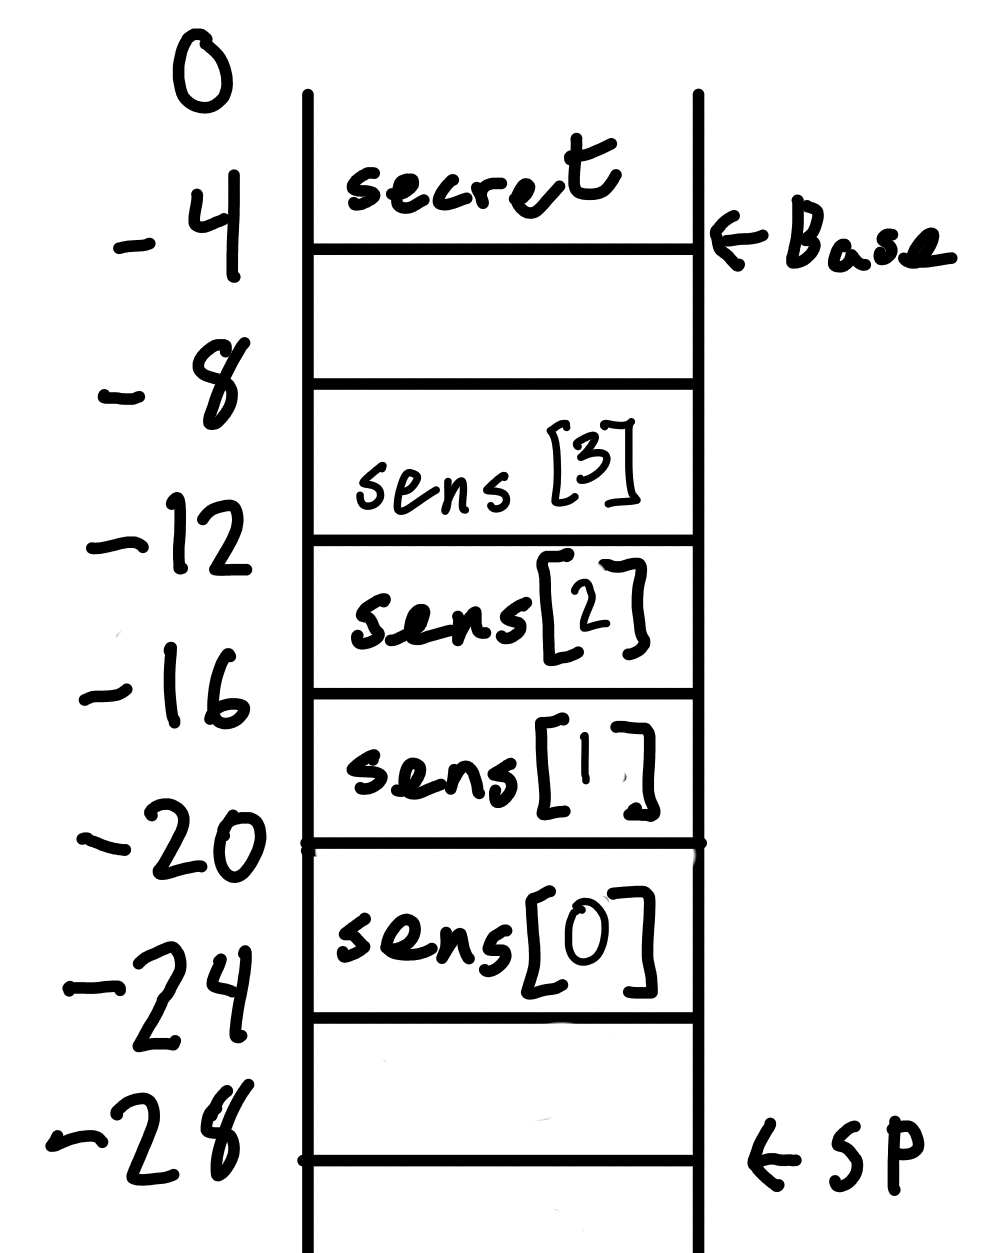
\includegraphics[width=\columnwidth]{stacklayout.png}
  \end{subfigure}

\caption{Example: Main}
\label{fig:main}
\end{figure}

\apt{C code, assembly code, and picture don't agree!
  Also, why aren't you showing the storing of ra on the stack as you do in 3(a)? (This is surely needed,
  and I think knowledgeable readers would expect it; anyhow, should be consistent across figures.)
  As a presentation thing: in the picture, offset labels on left should be positive, from sp, 0 through 24.}

Suppose that {\tt f} is not a (valid) C function at all, but an attacker seeking
to leak {\tt secret}! It might do so in a number of ways, shown as snippets of
assembly code in Figure \ref{fig:f}.\apt{explicitly reference the subfigure labels.}
It might take an offset from the stack
pointer, access {\tt secret}, and directly call {\tt publish} itself. But more
subtly, even if somehow prevented from outputting {\tt secret} directly, it might
instead return that value so that {\tt main} makes the call to {\tt publish}.
\apt{not what is happening in 3(b). (I'm not sure what is supposed to be happening there...)}

Beyond simply reading {\tt secret}, the attacker might overwrite {\tt sensitive[0]}
with 42, guaranteeing that {\tt main} publishes its own secret unintentionally!
Attacks of this kind do not violate {\tt main}'s confidentiality, but its
{\it integrity}.s
And last, but certainly not least, the attacker might attempt to return to the
wrong instruction, thereby bypassing the check and publishing {\tt secret} regardless,
violating the program's {\it well-bracketed control flow} (WBCF.)

\begin{figure}
  \begin{subfigure}[b]{.5\columnwidth}
    {\tt
      100: addi sp,sp,-4

      104: sw ra,4(sp)

      108: lw a0,20(sp)

      112: jal 88,ra

      116: lw ra,4(sp)

      120: jalr ra
    }
    \caption{Leaking {\tt secret} directly}
  \end{subfigure}  
  \begin{subfigure}[b]{.45\columnwidth}
    {\tt
      100: lw a4,16(sp)

      104: sw a4,12(sp)

      108: jalr ra
    }
    \caption{Leaking {\tt secret} indirectly}
  \end{subfigure}  
  
  \vspace{\belowdisplayskip}

  \begin{subfigure}[b]{.5\columnwidth}
    {\tt
      100: li a5,42

      104: sw a5,12(sp)

      108: jalr ra
    }
    \subcaption{Attacking {\tt sensitive}}
  \end{subfigure}
  \begin{subfigure}[b]{.45\columnwidth}
    {\tt
      100: addi ra,ra,20

      104: jalr ra
    }
    \subcaption{Attacking control flow}
  \end{subfigure}

  \caption{Assembly code for {\tt f} as an attacker}
  \label{fig:f}
\end{figure}

At the start of execution the program counter is 0 and the stack pointer -4, with code
proceeding upward\apt{don't need to say this}  and the stack growing down. The functions {\tt f} and {\tt publish}
are at addresses 100 and 200, respectively.\apt{not in the assembly code, they aren't!}

Figure \ref{fig:exec1} shows how the program counter, stack pointer, and call stack \apt{i.e. context?.
Confusing mix of real machine registers and abstract machine context.}
develop over several steps, with labels on the steps that allocate space and then make
a call. \(\downarrow \overline{\psi}\) in this diagram is a sideways
\(\xrightarrow{\overline{\psi}}\). Events are omitted.

\apt{It is difficult to track what is going on in thie figure with the original code; we have to keep
inspecting the pc. It would help to actually annotate the code with relevant security events.}
The first step  allocates a word for {\tt secret} and four for {\tt sensitive}. To
maintain a two-word alignment it leaves a gap.\apt{Not sure this is really what is
  going on in compiled code, but if so, rework to the example to avoid it, as we discussed!} This will have the
effect of marking those bytes \(\object\), assuming they were previously
\(\unsealed\).

\begin{figure*}
  \begin{subfigure}[t]{.5\textwidth}
    \vskip 0pt
    \begin{tabular}{| l | l | l | l |}
      \hline
      Step & \(\PCname\) & \(\SP\) & \(\context\) \\
      \hline
      0 & 0 & 0 & \(V_0, \emplist\) \\
      \hline
      \multicolumn{4}{l}{\(\downarrow [\mathbf{alloc} ~ (-4,4);\mathbf{alloc} ~ (-24,16)]\)} \\
      \hline
      1 & 4 & -24 & \(V_1 = V_0 \llbracket -24 \ldots -9, \mapsto \object \rrbracket\) \\
          & & & \(\llbracket -4 \ldots -1, \mapsto \object \rrbracket, \emplist\)\\
      \hline
      \multicolumn{4}{l}{\(\vdots\)} \\
      \hline
      4 & 16 & -24 & \(V_1, \emplist\) \\
      \hline
      \multicolumn{4}{l}{\(\downarrow [\mathbf{call} ~ 100 ~ \emplist ~ \emplist]\)} \\
      \hline
      5 & 100 & -24 & \(V_2 = V_1 \llbracket \reg \mapsto \unsealed | \reg \in \mathit{CLR} \rrbracket,\) \\
      & & & \([(V_1, 20, -24)]\) \\
      \hline
      \multicolumn{4}{l}{\(\vdots\)} \\
      \hline
      \(n\) & ? & ? & \(V_2,[(V_1, 20, -24)]\) \\
      \hline
      \multicolumn{4}{l}{\(\downarrow [\mathbf{return}]\)} \\
      \hline
      \(n+1\) & 20 & -24 & \(V_1, \emplist\) \\
      \hline
    \end{tabular}
  \end{subfigure}
  \begin{subfigure}[t]{.4\textwidth}
    \vskip 0px
    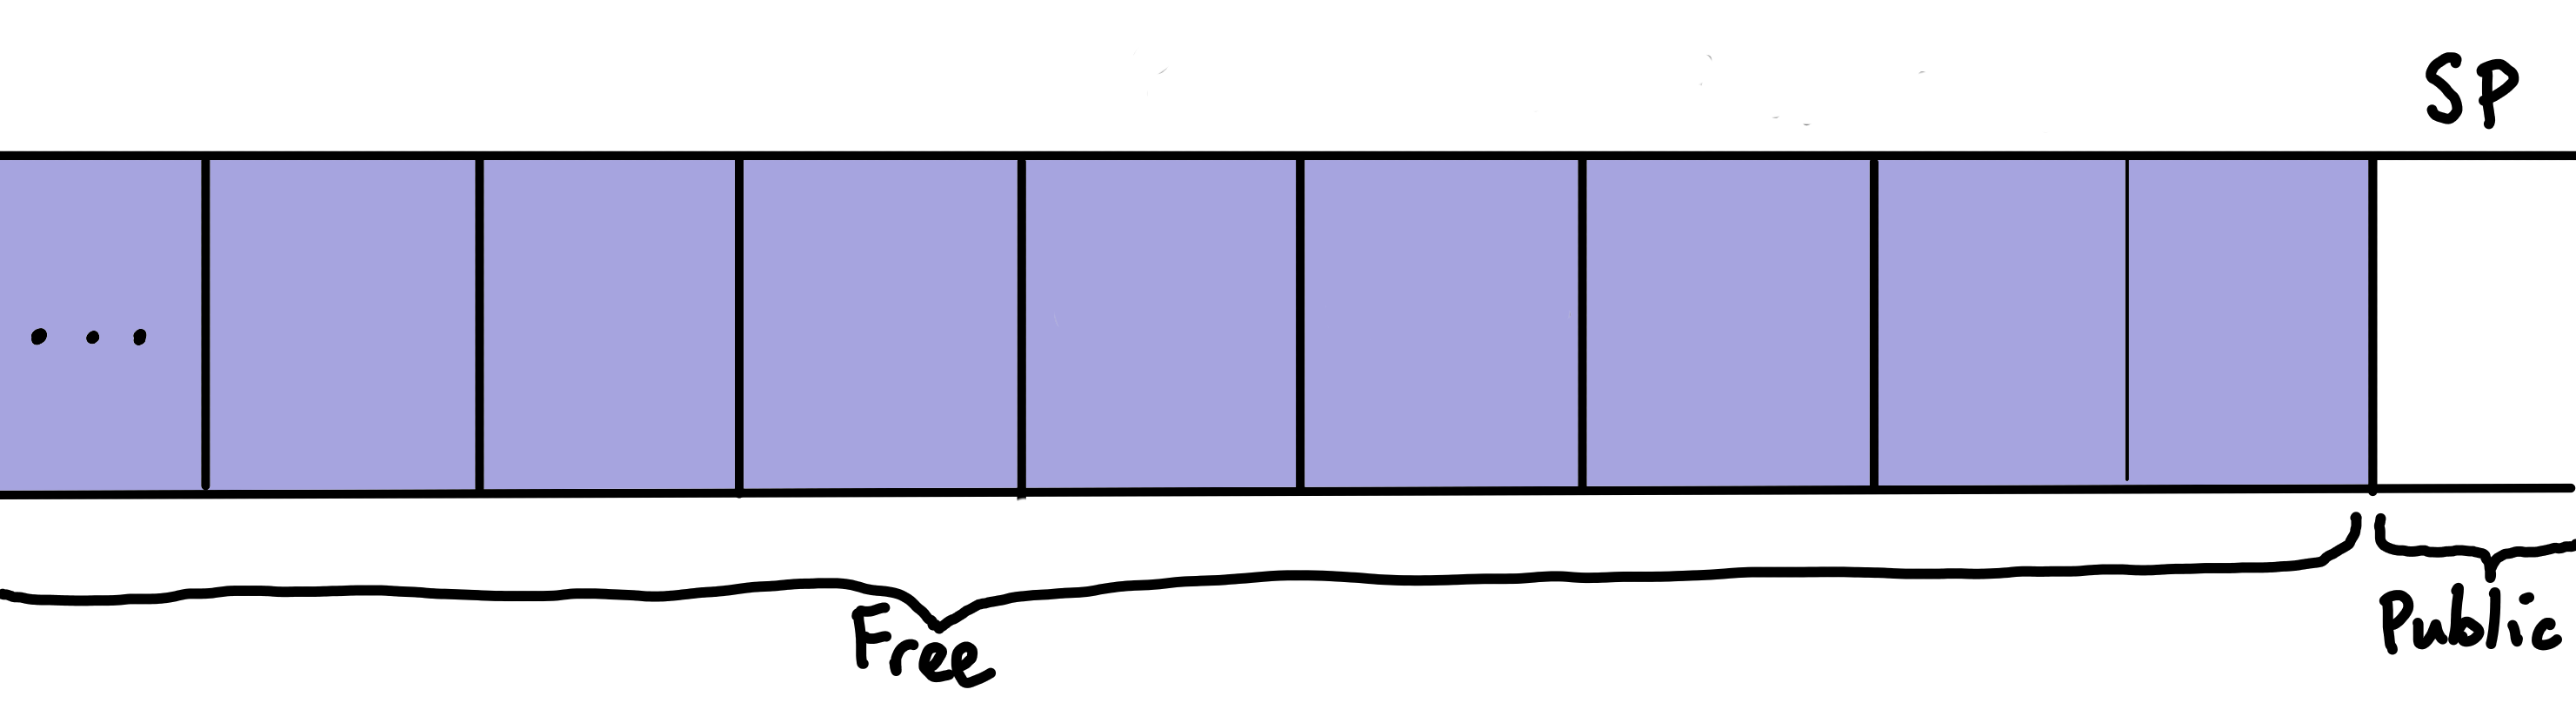
\includegraphics[width=\columnwidth]{stack1.png}
    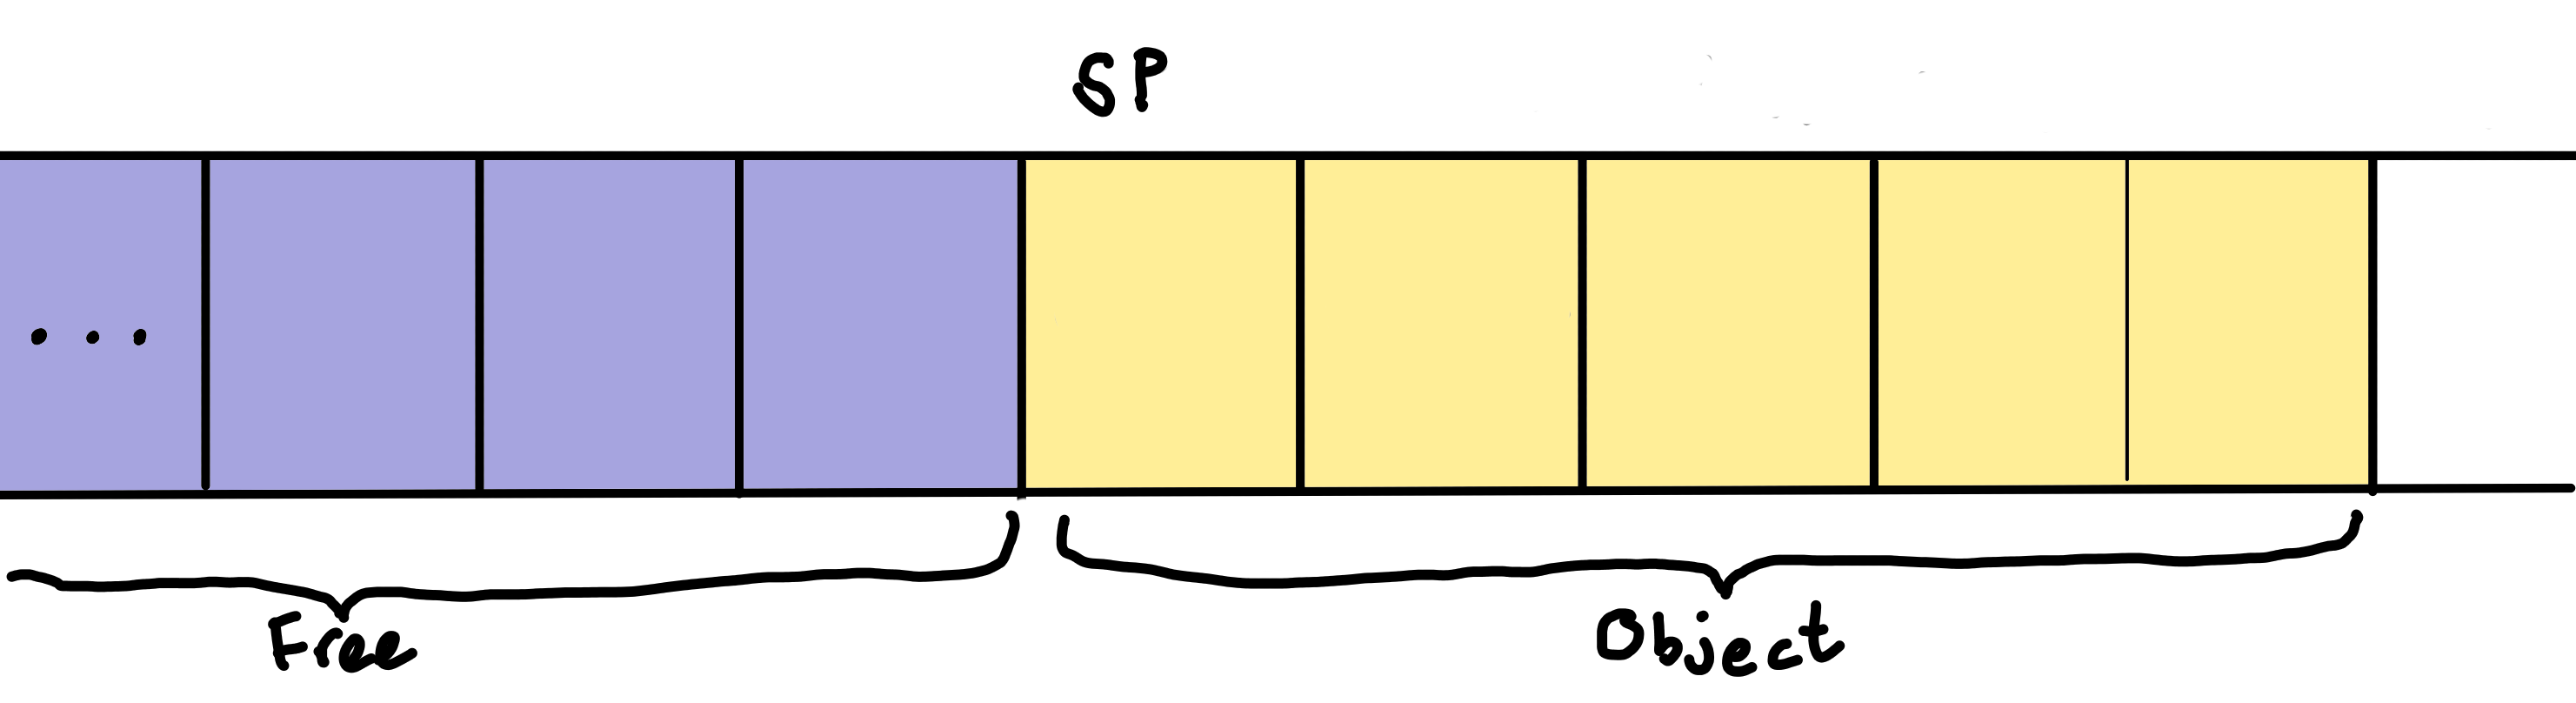
\includegraphics[width=\columnwidth]{stack2.png}
    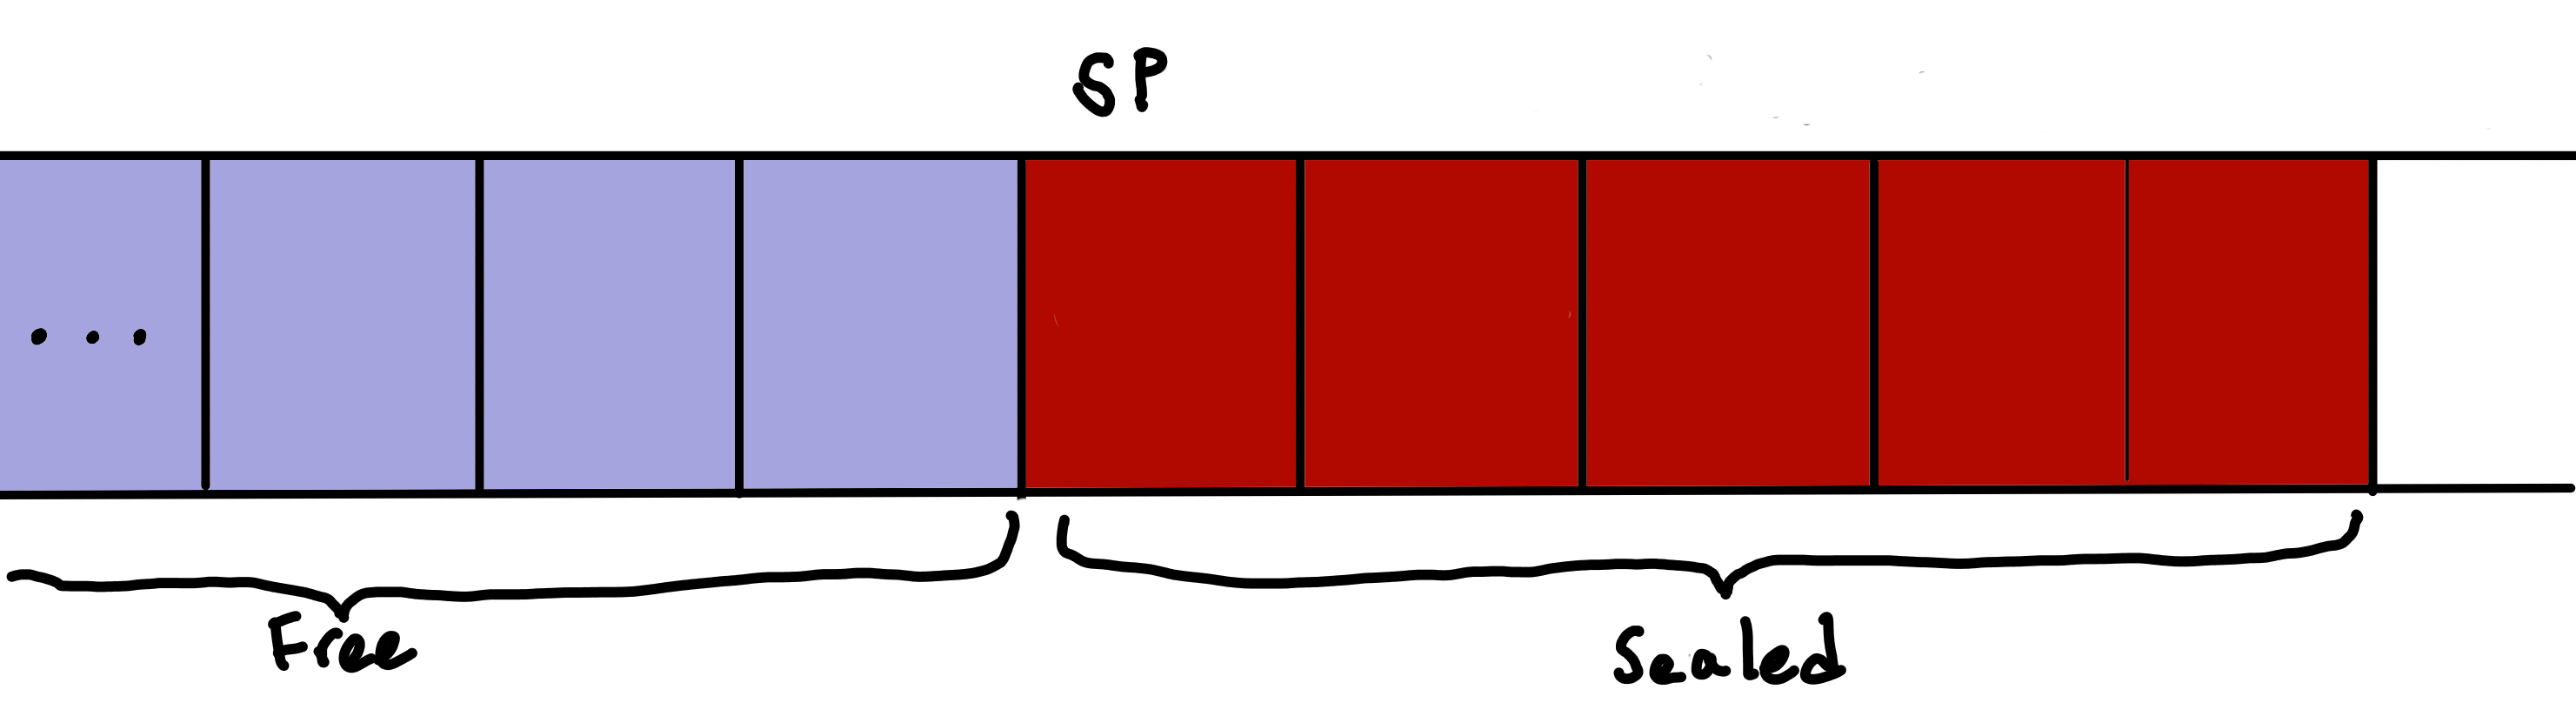
\includegraphics[width=\columnwidth]{stack3.png}
    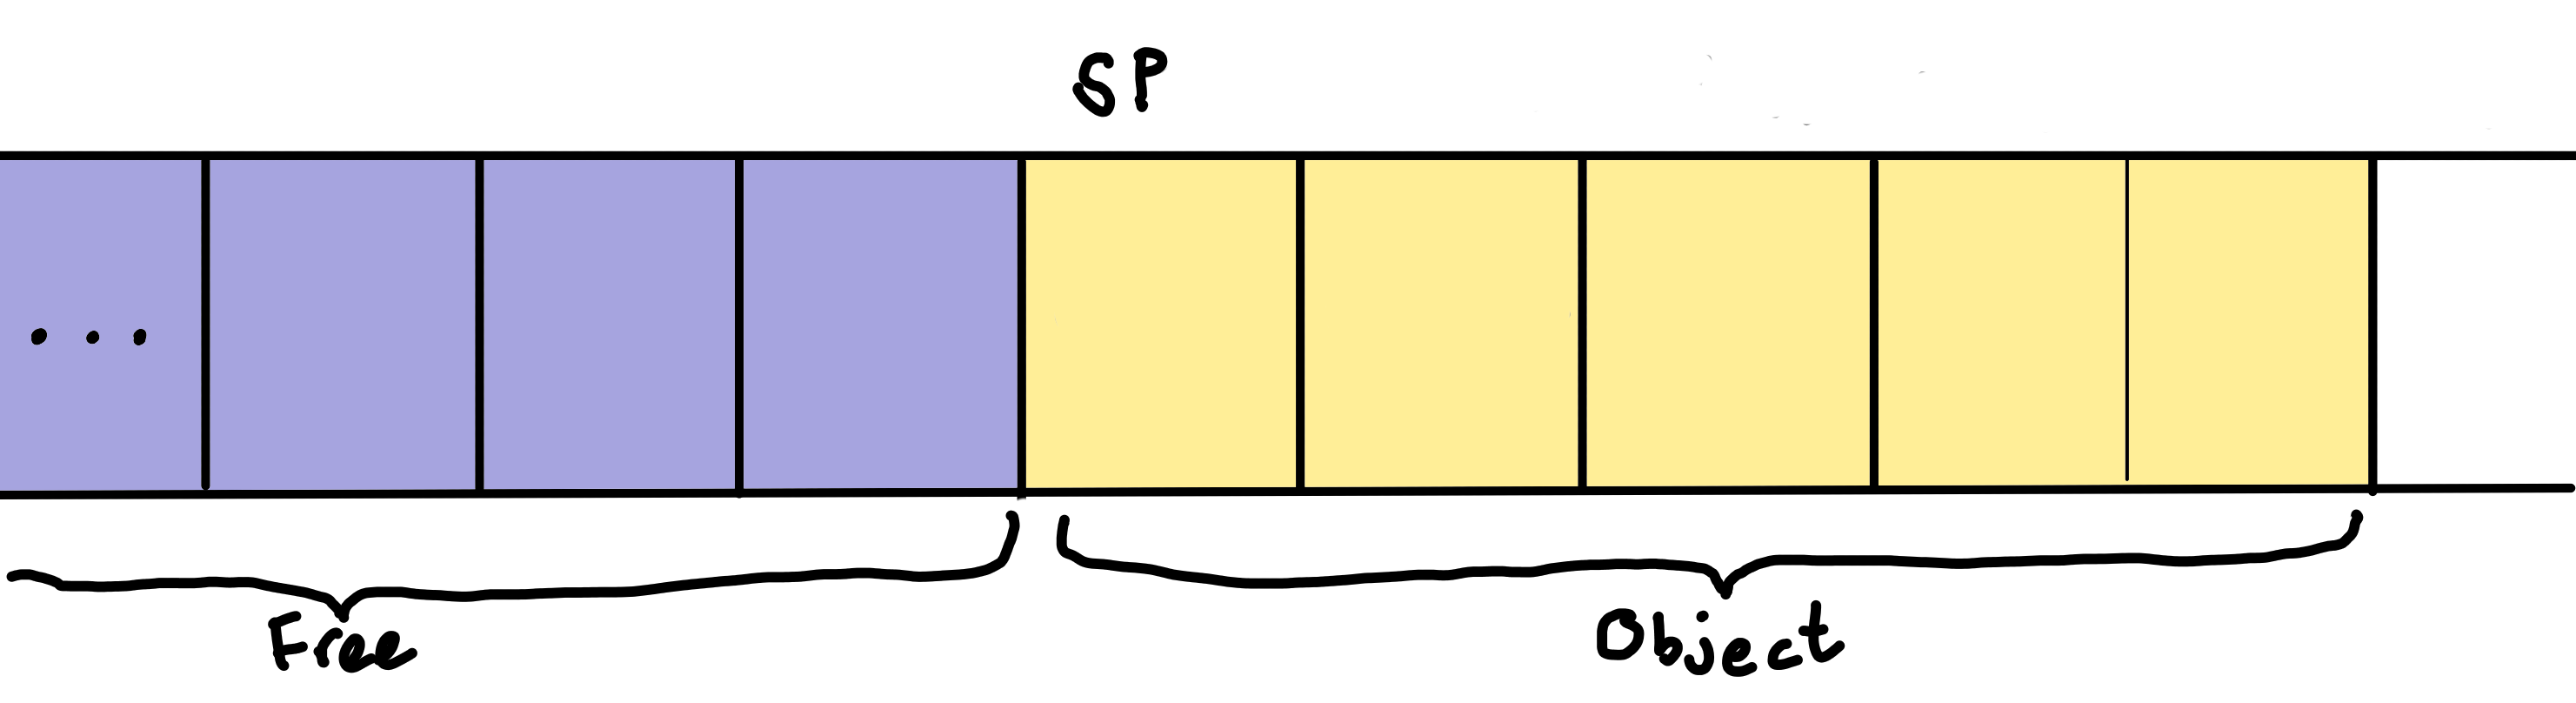
\includegraphics[width=\columnwidth]{stack4.png}
  \end{subfigure}

\caption{Execution through return from {\tt f}}
\label{fig:exec1}
\end{figure*}

On a call, the formerly active principal's record is pushed onto the inactive list.
Its return target is the return address of the call, 
and the stack pointer target is the stack pointer at the moment of call.
The callee's view is updated from the caller's such that the argument
registers are \(\public\) and any non-argument, caller-saved registers
are \(\unsealed\). All callee-save registers are always \(\sealed\) and
the program counter \(\public\), as they were initialized. \apt{Explain shat happens to
  $\object$s.}

We suppose that, on step \(n+1\), {\tt f} returns; if it does not, then
{\tt main}'s secrets are safe as long as {\tt f} does not leak them directly.
\apt{This is obscure. Are you talking about the jalr instruction serving as
  a return (and if not, why not?) or about the security label return? Why do
  you need to ``suppose'' anything; why not just show the code and explain that
it is annotated?}
On that return, we restore the topmost inactive principal, {\tt main}'s principal.
         
\paragraph*{Well-bracketed Control Flow}

But what if {\tt f} returns to an unexpected place (i.e. \(\PCname \neq 20\) or \(\SP \neq -24\)),
as would be the case in attack (d)? Then it has violated the WBCF property.
This property can be phrased in terms of a single step: for every transition
labeled as a return, the program counter and stack pointer at the next state
match those recorded in the top pending activation.

\paragraph*{Stack Integrity}

Integrity is more complicated, and requires us to compare the state at the start of
the call to {\tt f} to that on return. Intuitively, the integrity of {\tt main}
is preserved if, when control returns to it, it can rely on any \(\sealed\) elements
to be identical to when it made the call.

In the case of the call from {\tt main} to {\tt f}, the \(\sealed\) elements are the
addresses -24 through -9 and -4 through -1 (allocated as private data) and the callee-saved registers.
\apt{But there are no callee-saved registers in the example, so this is confusing. It would
  be easy enough to add one (e.g. to hold {\tt secret}), but probably better just to delay telling the
story about them until later.}
Note that the callee-saved registers may well have changed during the call -- but if
so, the callee is obligated to restore them to their prior value.

One further caveat: it is possible that {\tt f} might overwrite {\tt main}'s data
in a way that is harmless -- or that is rendered harmless by the enforcement mechanism!
This is the case in a lazy micro-policy: the monitor permits the caller to write into the
callee's frame, but taints that write so that the callee cannot read it later without
triggering a failstop. In such a scenario we will consider a value {\it harmless}\apt{Better, but I still
  think ``irrelevant'' would be better still. It is the write that is harmless, not the value.}
if it could be replaced with any other value without changing the observable behavior
of the machine. More precisely, for a given state \(\mach\) and set of elements \(\components\),
we define a {\em \(\components\)-variant} state to be one agrees with \(\mach\) on every element except those
in \(\components\). The elements of \(\components\) are said to be harmless in \(\mach\) if every
variant state produces an equivalent trace (see Section \ref{sec:events}.)

So, to define integrity, we need to know when a caller has been returned to;
this is the first state after the call in which the depth of the call stack
matches the state before the call. Integrity holds if, at that return state,
any element that is \(\sealed\) under the callee's view is either restored
to its original value or is harmless.
\apt{Can this be mapped map to the example?}
\paragraph*{Caller Confidentiality}

\apt{Remainder of this section is on the right track, but needs some expansion,
  and to be tied back more clearly and consistently to the examples. I started
  word-smithing this first para...}
We treat confidentiality as a form of non-interference as well: the confidentiality of a caller
means that its callee's behavior is dependent only on publicly visible data,
not the caller's private state. As we saw in the examples, we must consider both the observable events
that the callee produces during the call and the changes that the callee makes to the state that might
affect the caller after the callee returns.

Consider the state \((\mach, (V_2,\sigma))\) at step 5. If we take a variant state over
the set of element(s) that are \(\sealed\) or \(\unsealed\) in \(V_2\),
{\it internal confidentiality} means
that, if we execute both states until they return, they will produce equivalent sequences
of events.

But, it is also possible that the callee could extract data from the caller that it does
not use to produce a visible event, but instead stashes for later or uses to influence
its return value -- which in turn can lead to future changes in behavior that do not
even appear to be the fault of the callee!\apt{a bit repeetitious with above}
{\it Return-time confidentiality} means that any state element that changes in one variant
must either change in both, or be harmless. \apt{Explain this more! and tie back to examples.}

Together, these definitions encompass the confidentiality of the caller from the callee.

\paragraph*{Callee Confidentiality}

Although we presented our initial example from the perspective of the caller, a callee
may also have data that must be kept secret from its caller. Consider a callee that makes
a privileged system call to obtain a secret key, and uses that key to perform a specific
task. An untrustworthy or erroneous caller might attempt to read the key out of the callee's
memory after return.

We model this as nearly dual to caller integrity: the callee's secrets are those
values that it has stored in \(\unsealed\) elements. So, callee confidentiality means that
at the state following the callee's return, any element that was \(\unsealed\) under the
callee's view either retains its original value or is harmless.

\paragraph*{The Hierarchy of Stack Safety}

The forms of stack safety described above are largely independent of one another, and
can potentially be enforced separately in various combinations. This is important, because
many enforcement mechanisms already in existence only enforce some of the stack safety
properties. Stricter enforcement may have greater performance impacts, leading to decisions
about trade-offs between different points in a hierarchy of properties.

At the most basic, if we protect nothing else, it is vital to protect the control flow of the
system by enforcing WBCF. None of the data-protection properties are meaningful if a
callee can simply ``return'' to an arbitrary instruction and proceed with the privileges
of its caller! And from a practical standpoint, control-flow attacks such as return-oriented
programming are among the most severe attacks involving the stack and the core motivation
for much existing work.

\apt{Things sort of trail off here...Are there more interesting points on the hierarchy to discuss?
(And by the way, even WBCF needs to be loosened for exceptions.)}

\paragraph*{Moving Forward}

In the next section we will define traces and their (hyper-)properties.
Then in Section \ref{sec:facts} we will define a mechanism to make assertions
about what will happen on a future return, and Section \ref{sec:props} will use these
to give the formal definitions of integrity and confidentiality.

\section{Events and Traces}
\label{sec:events}

We abstract over the events that can be observed in the system, defining them
only as a set \(\OBSS\) that contains at least the element \(\tau\), the silent
event. Other events might represent certain function calls (i.e., system calls)
or writes to special addresses representing mmapped regions.
A {\em trace} is a nonempty, finite or infinite sequence
of events, ranged over by \(\obsT\).
We use ``\(\notfinished{}{}\)'' to represent ``cons'' for traces, reserving ``::''
for list-cons.

We write that execution from a state produces an observation trace
\(\mach,\context \hookrightarrow \obsT\) as follows, coinductively:

\judgmenttwo{\((\mach,\context) \stepstounder{} (\mach',\context',\obs)\)}
            {\((\mach',\context') \hookrightarrow \obsT\)}
            {\((\mach,\context) \hookrightarrow \notfinished{\obs}{\obsT}\)}

We define another relation that takes a trace until we have returned from the
active principal.
We write this \(d \downarrow (\mach,\context) \hookrightarrow \obsT\), where
\(d\) is the depth of the current call.

\judgment{\(|\sigma| < d\)}
         {\(d \downarrow (\mach,(V,\sigma)) \hookrightarrow \tau\)}

\judgmenttwobrlong{\((\mach,(V,\sigma)) \stepstounder{} (\mach',\context',\obs)\)}
                  {\(|\sigma| \geq d\)}
                  {\(d \downarrow (\mach',\context') \hookrightarrow \obsT\)}
                  {\(d \downarrow (\mach,(V,\sigma)) \hookrightarrow \notfinished{\obs}{\obsT}\)}

\paragraph*{Observational Similarity}

We say that two event traces $\obsT_1$ and $\obsT_2$ are {\em similar},
written \(\obsT_1 \eqsim \obsT_2\), if the sequence of non-silent events
is the same. That is, we compare up to deletion of \(\tau\) events.

\begin{minipage}{.4\columnwidth}
  \judgment{}{\(\obsT \eqsim \obsT\)}
\end{minipage}
\begin{minipage}{.4\columnwidth}
  \judgment{\(\obsT_1 \eqsim \obsT_2\)}
           {\(\notfinished{\obs}{\obsT_1} \eqsim \notfinished{\obs}{\obsT_2}\)}
\end{minipage}

\begin{minipage}{.4\columnwidth}
  \judgment{\(\obsT_1 \eqsim \obsT_2\)}
           {\(\notfinished{\tau}{\obsT_1} \eqsim \obsT_2\)}
\end{minipage}
\begin{minipage}{.4\columnwidth}
  \judgment{\(\obsT_1 \eqsim \obsT_2\)}
           {\(\obsT_1 \eqsim \notfinished{\tau}{\obsT_2}\)}
\end{minipage}

\paragraph*{Variants and Harmless Values}

Two states are variants with respect to a set of elements, \(\components\),
if they agree on the value of every element not in \(\components\). Our
notion of non-interference involves comparing the traces of such
\(\components\)-variants. We use this to define sets of vestigial\apt{oops. a meta-vestigial element!}  elements.

\definition Machine states \(\mach\) and \(\nach\) are {\em \(\components\)-variants},
written \(\mach \approx_\components \nach\), if, for
all \(\component \not \in \components\), \(\mach[\component] = \nach[\component]\).

\definition An element set \(\components\) in state \((\mach,\context)\) contains
harmless values, written \((\mach,\context) \parallel \components\), if for all
\(\nach\) such that \(\mach \approx_{\components} \nach\), if 
\((\mach,\context) \hookrightarrow \obsT\) and
\((\nach,\context) \hookrightarrow \obsT'\), then
\(\obsT \eqsim \obsT'\).

\section{Facts Abouts Calls and Returns}
\label{sec:facts}

Here we define some logical operations to reason about the behavior of the
system over time. These have a temporal-logic flavor, as they reflect
the expected behavior of the system in the future, after a possible return.

\paragraph*{On-return}

The intuition behind integrity (below) is that a caller may expect its
sealed data to be unchanged when control returns to it. In fact, the callee
may overwrite such data -- when the data are found in callee-saved registers
this is perfectly legal -- as long as it either restores it, or has some guarantee
that its changes will not impact the caller.

We start by defining a second-order logical operator
\(d \uparrow P\), read ``\(P\) holds on return from depth \(d\),''
where \(P\) is a predicate on machine states. This is a coinductive relation
similar to ``weak until'' in temporal logic -- it holds if the program never
returns from depth \(d\).

\judgmenttwo[Returned]
            {\(|\sigma| < d\)}
            {\(P ~ (\mach,(V,\sigma))\)}
            {\((d \uparrow P) ~ (\mach, (V,\sigma))\)}

\judgmenttwobrlong[Step]
                  {\(|\sigma| \geq d\)}
                  {\((d \uparrow P) ~ (\mach', \context')\)}
                  {\((\mach, (V,\sigma)) \stepstounder{\overline{\psi}} (\mach', \context',\obs)\)}
                  {\((d \uparrow P) ~ (\mach, (V,\sigma))\)}

Similarly, in confidentiality, we will want to compare pairs of future states,
so we give a binary equivalent, \(d \Uparrow R\), so that
\((\mach,\context) ~ (d \Uparrow R) ~ (\mach',\context')\) holds if \(R\) holds on the
first states that return from depth \(d\) after \((\mach,\context)\) and \((\mach',\context')\).
Once again, \(\Uparrow\) is coinductive.

\judgmenttwobrlong[Returned]
            {\(|\sigma_1| < d\)}
            {\(|\sigma_2| < d\)}
            {\((\mach_1,(V_1,\sigma_1)) ~ R ~ (\mach_2,(V_2,\sigma_2))\)}
            {\((\mach_1,(V_1,\sigma_1)) ~ (d \Uparrow R) ~ (\mach_2,(V_2,\sigma_2))\)}

\judgmenttwobrlong[Left]
              {\(|\sigma_1| \geq d\)}
              {\((\mach_1,(V_1,\sigma_1)) \stepstounder{\overline{\psi}} (\mach_1',\context_1',\obs)\)}
              {\((\mach_1',\context_1') ~ (d \Uparrow R) ~ (\mach_2,(V_2,\sigma_2))\)}
              {\((\mach_1,(V_1,\sigma_1)) ~ (d \Uparrow R) ~ (\mach_2,(V_2,\sigma_2))\)}

\judgmenttwobrlong[Right]
              {\(|\sigma_2| \geq d\)}
              {\((\mach_2,(V_2,\sigma_2)) \stepstounder{\overline{\psi}} (\mach_2',\context_2',\obs)\)}
              {\((\mach_1,(V_1,\sigma_1)) ~ (d \Uparrow R) ~ (\mach_2,\context_2')\)}
              {\((\mach_1,(V_1,\sigma_1)) ~ (d \Uparrow R) ~ (\mach_2,(V_2,\sigma_2))\)}

\section{Properties}
\label{sec:props}

We now finally have everything we need to offer our definitions for stack safety.
Figure \ref{fig:oprules} gives the operation rules for all of the operations we've described
so far.

\begin{figure}

  \judgmentbr[Alloc]
             {\(b = \mach[\SP] + \mathit{off}\)}
             {\(V' = V \llbracket \addr \mapsto \sealed |
               b \leq a < b+\mathit{sz} \land V ~ \addr = \unsealed \rrbracket\)}
             {\(Op ~ (\mathbf{alloc} ~ \mathit{off, sz}) ~ (V,\sigma) ~ \mach = (V',\sigma)\)}

  \judgmentbr[Call]
             {\(\psi = \mathbf{call} ~ \addr_{target} ~ \overline{\reg_{args}} ~ \overline{sa}\)}
             {\(V' = V \llbracket \reg \mapsto \unsealed | \reg \in \mathit{CLR} \rrbracket
               \llbracket \reg \mapsto \public | \reg \in \overline{\reg_{args}} \rrbracket\)}
             {\(Op ~ \psi ~ (V,\sigma) ~ \mach =
               (V',(V, \mach[\PCname]+4, \mach[\SP])::\sigma)\)}

  \judgment[Ret]
           {\(\sigma = (V,\addr_{ret},\addr_{sp})::\sigma'\)}
           {\(Op ~ \mathbf{return} ~ (\_, \sigma) ~ \mach = (V, \sigma)\)}
           
%\judgment[RetDef]
%         {\(\chi = \mathbf{return}\)}
%         {\(Cop ~ \chi ~ (V, \emplist) ~ \mach \triangleq
%           (V, \emplist)\)}

  \caption{Core operation rules for the simple system}
  \label{fig:oprules}
\end{figure}

\subsection{Well-bracketed Control Flow}

\definition A system enjoys well-bracketed control flow if, for all states
\((\mach,(\_,(\_,\addr_{ret},\addr_{sp})) \stepstounder{\mathbf{return}} (\mach',\context)\),
\(\mach'[\PCname] = \addr_{ret}\) and \(\mach'[\SP] = \addr_{sp}\).

\subsection{Integrity}

\definition Let \(\Delta(\mach,\mach')\) be the set of elements \(\component\)
such that \(\mach[\component] \not = \mach'[\component]\).

\definition Let \((\mach,\context)\) be a combined state with
\(\context = (V,\sigma)\), and
\(\components = \{\component | V ~ \component = \sealed\}\).
Let \(P\) be a predicate that holds on a state \((\mach',\context')\) if
\(\mach' ~ \parallel ~ \Delta(\mach,\mach') \cap \components\).
Then \(\mach\) enjoys {\it return-time integrity} if \(|\sigma| \uparrow P\) holds
on \((\mach,\context)\).

\definition A system enjoys {\it stack integrity} if, for all reachable states
\((\mach,\context)\) such that
\((\mach,\context) \stepstounder{\overline{\psi}} (\mach',\context',\obs)\) with
\(\mathbf{call} ~ \addr ~ \overline{\reg} \in \psi\) or
\(\mathbf{tailcall} ~ \addr ~ \overline{\reg} \in \psi\),
\((\mach',\context')\) enjoys return-time integrity.

\subsection{Caller Confidentiality}

\definition The {\em corrupted set} \(\bar{\Diamond}(\mach,\mach',\nach,\nach')\)
of four states treats \(\mach\) and \(\nach\) as the initial states and
\(\mach'\) and \(\nach'\) as their corresponding final states, and is the
set of elements that were corrupted between them. That is, the set of all elements
\(\component \in \Delta(\mach,\mach') \cup \Delta(\nach,\nach')\) such that
\(\mach'[\component] \not = \nach'[\component]\).

\definition Let \((\mach,\context)\) be a state with \(\context = (V,\sigma)\), and
\(\components = \{\component | V ~ \component \in \{\sealed, \unsealed\}\}\).

Then \((\mach,\context)\) enjoys {\it internal confidentiality} with respect to
if, for any \(\nach\) that is a \(\components\)-variant of \(\mach\), we can take
\(|\sigma| \uparrow (\mach,\context) \hookrightarrow \obsT\) and
\(|\sigma| \uparrow (\nach,\context) \hookrightarrow \obsT'\) and have that
\(\obsT \simeq \obsT'\).

\definition Let \((\mach,\context)\) be a state with \(\context = (V,\sigma)\),
and \(\components = \{\component | V ~ \component \in \{\sealed, \unsealed\}\}\).
Let \(\nach\) be a \(\components\)-variant of \(\mach\).
Let \(R\) be a relation such that \((\mach_1,\context_1) ~ R ~ (\mach_2,\context_2)\)
if \(\bar{\Diamond}(\mach,\mach_1,\nach,\mach_2)\) is harmless in \((\mach_1,\context_1)\).
Then \((\mach,\context)\) enjoys {\it return-time confidentiality}
if, for any such \(\nach\), \((\mach,\context) ~ (|\sigma| \Uparrow R) ~ (\nach,\context)\).

\definition A system enjoys {\it caller confidentiality} if, for all reachable states
\((\mach,\context)\) such that
\((\mach,\context) \stepstounder{\overline{\psi}} (\mach',\context',\obs)\)
with \(\mathbf{call} ~ \addr ~ \overline{\reg} \in \psi\) or
\(\mathbf{tailcall} ~ \addr ~ \overline{\reg} \in \psi\),
\((\mach',\context')\) enjoys both internal and return-time confidentiality.

\subsection{Callee Confidentiality}

\definition Let \((\mach,\context)\) be a state with \(\context = (V,\sigma)\), and
\(\components = \{\component | V ~ \component = \unsealed\}\).
Let \(P\) be a predicate that holds on a state \((\mach',\context')\) if
\(\mach' ~ \parallel ~ \Delta(\mach,\mach') \cap \components\).
Then \(\mach\) enjoys {\it post-return confidentiality} if \(|\sigma| \downarrow P\) holds.

\definition A system enjoys {\it callee confidentiality} if, for all reachable states
\((\mach,\context)\) such that \((\mach,\context) \stepstounder{\overline{\psi}} (\mach',\context',\obs)\)
with \(\mathbf{call} ~ \addr ~ \overline{\reg} \in \psi\) or
\(\mathbf{call} ~ \addr ~ \overline{\reg} \in \psi\),
\((\mach',\context')\) enjoys post-return confidentiality
with respect to \(\context\).

\section{Shared Memory}

%We can extend our basic machine to support public memory allocations that can
%be accessed by anyone until they are deallocated on their owner's return,
%using the \(\mathbf{alloc\_pub}\) operation. This behaves identically to
%\(\mathbf{alloc\_priv}\) except that it marks the locations \(\public\).
%For example, consider the following code:

%{\tt
%  void g() \{

%  ~ ~ int x[3];

%  ~ ~ int y;

%  ~ ~ h(\&x);
    
%  \}
%}

%Here we have allocated several arrays and variables; {\tt y}
%will behave as normal with \(\mathit{alloc\_priv}\), but {\tt x} has its
%address taken and passed to another function. That function might do anything at
%all to {\tt x}, and we have to decide whether it can be said to violate stack
%safety. A reasonable default is to assume that any address-taken local should be
%public, while {\tt y} is still private.

%In the likely event that the space for the return address, {\tt x}, and {\tt y}
%are all allocated in a single step, that step needs multiple labels to capture
%that they are not all private. Its label would instead be:
%\[\begin{split}
%& \psi = [\mathbf{alloc\_priv} ~ (20,4); \\
%  & \mathbf{alloc\_pub} ~ (16,12) ; \mathbf{alloc\_priv} ~ (4,4)]
%\end{split}\]

%Allocating public objects affects the call stack very similarly to private ones,
%but instead of treating them as \(\sealed\) they become \(\public\). This makes these
%regions of memory able to transmit information between caller and callee without
%violating the stack safety properties. Note that there is no way to seal a location
%once it has become \(\public\); only when {\tt g} returns will the memory allocated
%to {\tt x} be available for private use.

%\judgmentbr{\(b = \mach[\SP] - \mathit{off}\)}
%           {\(V' = V \llbracket \addr \mapsto \public |
%             b \leq a < b+\mathit{sz} \land V ~ \addr = \unsealed \rrbracket\)}
%           {\(Pop ~ (\mathbf{alloc\_pub} ~ \mathit{off, sz}) ~ (V,\sigma) ~ \mach \triangleq
%             (V',\sigma)\)}

\subsection{Stack Arguments}

So far, we have not dealt with arguments spilled onto the stack, variadic arguments,
or arguments that are passed by reference without their addresses being taken
explicitly (i.e., structs and arrays passed directly.) Consider the simplest case,
where a function has more than 8 arguments and therefore must (in RISC-V) spill one
to the stack.

\begin{minipage}[t]{.6\columnwidth}
{\tt
  void main() \{

  ~ f(1,2,3,4,5,6,7,8,9);

  ~ g(42);
  
  \}
}
\end{minipage}
\begin{minipage}[t]{.35\columnwidth}
{\tt
0: addi sp,sp,-24

4: sd ra,16(sp)

8: li a5,9

12: sd a5,0(sp)

16: li a7,8

...

48: jal 52,ra

52: li a0,42

56: jal 144,ra
}
\end{minipage}

Under a typical calling convention, the callee expects the ninth argument to
be passed to it at the stack pointer, so the caller places it there
{\it without moving the stack pointer}. We model this by labeling the transition
from instruction 48 as a call {\it followed by an allocation}.
\([\mathbf{call} ~ 100 ~ [\mathtt{ra0-ra7}]; \mathbf{alloc} ~ (0,4)]\).

This has the effect of first pushing a new view onto the call stack, then
updating the callee's view so that the word following the stack pointer is
already marked \(\object\).

So, we first apply \(Op ~ (\mathbf{alloc} ~ (0,4))\) and mark that region as
\(\object\). But we do not want to seal it when we make the call! So we must
refine our call operation to make use of the information that we have about
which stack offsets contain arguments, \(\overline{sa}\). We first define the
helpful set \(\mathit{passed} ~ \overline{sa} ~ \mach\) based on those offsets,
then extend the call operation to keep all objects in \(\mathit{passed}\) marked
as \(\object\) and seal everything else.
%
\[\mathit{passed} ~ \overline{sa} ~ \mach \triangleq
\bigcup_{(b,o) \in \overline{sa}} \{\mach[\SP]+i | b \leq i < b+o\}\]
%
\judgmentbrbr[]
             {\(\psi = \mathbf{call} ~ \addr_{target} ~ \overline{\reg_{args}} ~ \overline{sa}\)}
             {\(V' = V \llbracket \reg \mapsto \unsealed | \reg \in \mathit{CLR} \rrbracket
               \llbracket \reg \mapsto \public | \reg \in \overline{\reg_{args}} \rrbracket\)}
             {\(V'' = V'\llbracket \addr \mapsto \sealed | V' ~ \addr = \object \land \addr \not \in (\mathit{passed} ~ \overline{sa} ~ \mach) \rrbracket\)}
             {\(Op ~ \psi ~ (V,\sigma) ~ \mach =
               (V',(V, \mach[\PCname]+4, \mach[\SP])::\sigma)\)}

The remaining definitions are unchanged. Now a stack-spilled argument can be allocated
and remain accessible in the callee, while its memory is sealed for calls that do not
use that memory as an argument.

\subsection{Pass-by-reference}

[Still to-do]

\subsection{Provenance, Capabilities, and Protecting Objects}

What if we want to express a finer-grained notion of safety, in which
such objects are protected unless the function that owns them intentionally
passes a pointer to them?

In order to express such a property, we need our machine to carry some notion
of {\it pointer provenance} -- a distinction between a pointer that is intended to
point to a given object, and non-pointer integers as well as pointers to other objects.
Then \(\mathit{passed}\) should recursively identify all objects that
are reachable transitively from valid pointers in registers and accessible memory;
these keep their \(\object\) status, while those that are not reachable become \(\sealed\).
         
\bibliographystyle{IEEEtran}
\bibliography{bcp.bib,local.bib}

\end{document}
